\documentclass[10pt,a4paper]{article}
\usepackage[margin=2.1cm]{geometry}
\usepackage{amsmath,amssymb}
\usepackage{booktabs}
\usepackage{graphicx}
\usepackage{float}
\usepackage{caption}
\usepackage{subcaption}
\usepackage{xcolor}
\usepackage{hyperref}
\usepackage{natbib}
\usepackage{microtype}
\usepackage{array}
\usepackage{tabularx}
\usepackage{url}
\graphicspath{{figures/}}
\hypersetup{colorlinks=true,linkcolor=blue,citecolor=blue,urlcolor=blue}
\setlength{\parskip}{0.35em}
\setlength{\parindent}{0pt}
\captionsetup{font=small,labelfont=bf}
\newcommand{\code}[1]{\texttt{#1}}

\title{\vspace{-1.4cm}\textbf{DSA5208 Project 3}\\Parallel K-Means on Covertype: Strong, Weak and Hybrid Scaling on Vanda}
\author{[Team Member 1: Name, Student ID] \and [Team Member 2: Name, Student ID]}
\date{November 2026}

\begin{document}
\maketitle

\begin{abstract}
We evaluate serial, OpenMP, MPI, hybrid MPI+OpenMP and GPU implementations of Lloyd's K-means on UCI Covertype ($N=581{,}012$, $D=54$, $K=7$). On top of the dataset, this project uses deterministic resampling to create larger workloads. On the original dataset, MPI strong scaling reaches 129.7$\times$ speedup at 256 ranks (50.7\% efficiency) on a four-node allocation, and weak scaling retains 80.2\% efficiency. The 10M strong-scaling extension reaches approximately 133.0$\times$ (52.0\%). A Vanda OpenMP sweep reaches approximately 24.2$\times$ at 64 threads on the original dataset. At 256 total workers, six unpinned 10M hybrid layouts range from 0.489 to 0.599 seconds; a separate pinned 256$\times$1 recovery completed at 0.32014 seconds, and is reported with its different allocation and binding rather than as a same-allocation control. Separate placement experiments expose substantial collective-time sensitivity, while a pinned 256$\times$1 baseline rerun is stable. NVIDIA A40 assignment kernels are fast but CPU accumulation limits end-to-end GPU performance. Real-data clustering does not reproduce the seven cover-type labels (ARI 0.022, NMI 0.065). We distinguish complete measured evidence from failed or pending jobs throughout, and a dedicated section analyses the practical difficulties of repeatedly obtaining 256-core allocations.
\end{abstract}

\section{Introduction}
K-means \citep{lloyd1982,macqueen1967} is a canonical data-mining workload, but its parallel behaviour is
more subtle than the assignment kernel suggests. This project investigate how well the algorithm scales on a
real cluster, where the communication and placement costs appear, and whether
hybrid MPI+OpenMP or a GPU improves the end-to-end fit.

The conditions are:
\begin{itemize}
\item a controlled serial and MPI scaling study on Vanda up to 256 CPU cores;
\item a separate 4$\times$64 versus 8$\times$32 topology comparison, reported
      as a hardware/placement observation rather than a node-count law;
\item a repaired Hybrid analysis that separates invalid unpinned runs from a
      valid five-repetition pinned-core experiment;
\item a CUDA A40 evaluation with transfer, kernel, accumulation and end-to-end
      timings kept distinct;
\item a real-data Covertype interpretation using only the original 581,012
      observations.
\end{itemize}

\section{Dataset and preprocessing}
Covertype \citep{blackard1999} contains 581,012 observations, 54 predictive
features and seven forest-cover classes. The first ten features are
quantitative (elevation, aspect, slope, hydrology, road and fire distances,
hillshade); the remaining 44 are binary wilderness and soil indicators. The
class label is column 55 and is excluded from clustering.

The first ten features are z-scored with the population standard deviation;
zero-variance columns map to zero. The 44 binary indicators remain 0/1. The
same transformation, feature order, seed (42) and K-means++ initialization
\citep{arthur2007} are used by every CPU implementation. The class-ordered file
is read with systematic subsets for the serial size sweep, so class
proportions are not distorted by taking the first rows. The resampled
weak-scaling workload repeatedly samples real Covertype rows; it is benchmark
data, not new forest observations.

\section{K-means algorithm}
For observations $x_i\in\mathbb{R}^{D}$ and centroids $c_k$, squared Euclidean
distance is
\begin{equation}
d^2(x_i,c_k)=\sum_{j=1}^{D}(x_{ij}-c_{kj})^2 .
\end{equation}
Assignment selects the nearest centroid, with ties broken by the lowest
cluster id:
\begin{equation}
a_i=\arg\min_{k\in\{0,\ldots,K-1\}} d^2(x_i,c_k).
\end{equation}
For each cluster, the local sums and counts are
\begin{equation}
S_k=\sum_{i:a_i=k}x_i,\qquad n_k=\sum_{i:a_i=k}1,
\end{equation}
and the update is
\begin{equation}
c_k=\begin{cases}S_k/n_k,&n_k>0,\\ c_k,&n_k=0,\end{cases}
\end{equation}
i.e.\ an empty cluster retains its previous centroid. The objective is
\begin{equation}
\mathrm{SSE}=\sum_{i=1}^{N}d^2(x_i,c_{a_i}).
\end{equation}
The measured convergence rule is zero changed labels over the full dataset;
fixed-iteration runs execute exactly $I=30$ iterations for performance
comparability.

\begin{figure}[H]
\centering
\begin{minipage}{0.93\textwidth}
\small
\begin{verbatim}
initialise K centroids by K-means++ (seed 42)
for iter = 1..I:
    zero local sums S_k and counts n_k
    for each local observation x_i:
        a_i = argmin_k ||x_i - c_k||^2      # lowest id breaks ties
        n_{a_i} += 1
        S_{a_i} += x_i
    allreduce S (K*D doubles) and n plus changed count (K+1 uint64)
    for k = 0..K-1:
        if n_k > 0: c_k = S_k / n_k          # empty cluster keeps c_k
    if global changed labels == 0: stop
\end{verbatim}
\end{minipage}
\caption{Parallel Lloyd iteration used by all CPU implementations. The
assignment and local accumulation are local; the two \code{MPI\_Allreduce}
operations are the synchronization points.}
\label{fig:pseudocode}
\end{figure}

\paragraph{Complexity.}
Each iteration evaluates $N K$ distances of dimension $D$, giving
$O(I N K D)$ arithmetic and $O(NKD)$ serial memory traffic when the data are
streamed. The global reduction carries only $K D$ doubles and $K+1$ integers
per rank, so its \emph{volume} is small ($8KD+8(K+1)=3{,}088$ bytes for
$K=7,D=54$), while its \emph{latency} and synchronization cost grow with rank
count. This is why K-means is data-parallel but not embarrassingly parallel:
the assignment is local, the centroid update is global.

\section{Parallelization design}
\subsection{Serial and OpenMP}
The serial kernel fuses assignment, count and sum accumulation in one pass over
the row-major matrix. The OpenMP \citep{dagum1998} kernel parallelizes that pass with
\code{\#pragma omp for schedule(static)}. Every thread owns a private
$K\times D$ sum array and $K$ counts, avoiding atomics and false sharing of the
rank-level arrays. The main thread folds the private arrays in fixed thread-id
order, so a fixed team size gives a deterministic reduction; only after the
fold does the centroid update run.

\subsection{MPI}
The MPI implementation follows the message-passing model \citep{mpiforum2015}. Observations are partitioned into contiguous blocks. With $P$ ranks,
\code{base = N/P} and the first $N\bmod P$ ranks take one extra row. Each rank
computes local sums and counts, then calls two collectives per iteration:
\code{MPI\_Allreduce} of $K D$ doubles for sums and \code{MPI\_Allreduce} of
$K+1$ \code{uint64} values for counts plus the changed-label count. Every rank
receives the same totals and updates the same centroids. The fit time is the
maximum elapsed time across ranks; phase maxima are reported separately and are
never added to claim a total.

\subsection{Hybrid MPI+OpenMP}
The hybrid program uses the MPI decomposition with an OpenMP team inside each
rank. Thread-local arrays are folded into rank-local totals in fixed thread-id
order; the main thread performs both MPI reductions. \code{MPI\_Init\_thread}
requests \code{MPI\_THREAD\_FUNNELED} and the program verifies the provided
level. This is the correct level because only the main thread calls MPI.

At a fixed 64-core budget, the rank/thread layouts trade collective traffic
against OpenMP synchronization. Fewer ranks reduce the number of participants
in each Allreduce, but each rank has a larger OpenMP team and a larger local
fold/barrier. The measured 64-core comparison in Section~\ref{sec:hybrid}
quantifies that trade-off rather than assuming Hybrid should win.

\subsection{GPU design}
The CUDA \citep{nickolls2008} implementation keeps the K-means logic on the host and runs only the
nearest-centroid assignment on the A40. The centroid matrix ($7\times54$
floats) is placed in constant memory. Stage~A re-uploads the observation matrix
every iteration and reads labels back; Stage~B keeps the matrix resident and
re-uploads only centroids. Device arithmetic is float32, while host sums,
counts, centroid updates and the reference implementation remain float64. The
in-process CPU reference uses the same initialization and iteration count, so
GPU label agreement, centroid difference and inertia difference are measured
rather than assumed. Apple Metal follows the same staging on an M1 Pro; it is
reported as a separate platform, not as a Vanda result.

\section{Experimental setup and methodology}
\subsection{Hardware and software}
Table~\ref{tab:hardware} lists the environments. All primary Vanda runs use
GCC 11.4/11.5, OpenMPI 4.1.8 and \code{-O3 -std=c++17 -DNDEBUG}. The Vanda
jobs use PBS Pro; the 4$\times$64 jobs request four 64-core chunks
(\code{select=4:ncpus=64}), the 8$\times$32 jobs eight 32-core chunks, and the
single-node jobs one 64-core chunk. Atlas is included only as historical
cross-platform context.

\begin{table}[H]
\centering\small
\caption{Environments used by the committed results. The 4$\times$64 and
8$\times$32 Vanda jobs differ in node family as well as node count.}
\label{tab:hardware}
\begin{tabular}{llll}
\toprule
Environment & Shape & CPU / device & Toolchain \\
\midrule
Vanda GN-A40 & 4 nodes $\times$ 64 cores & Xeon Platinum 8452Y & GCC 11.5, OpenMPI 4.1.8 \\
Vanda CN & 8 nodes $\times$ 32 cores & Xeon Platinum 8452Y & GCC 11.4, OpenMPI 4.1.8 \\
Vanda IN & 1 node $\times$ 64 cores & Xeon Gold 6438N & GCC 11.4, OpenMPI 4.1.8 \\
Vanda A40 & 1 GPU + host & NVIDIA A40, sm\_86 & CUDA 12.x, GCC 11.5 \\
Atlas (historical) & 1 node $\times$ 96 cores & AMD EPYC 7R13 & GCC 7.3, OpenMPI 4.1.1 \\
Apple M1 Pro & 8 cores + GPU & Apple M1 Pro & Apple clang 21, Metal \\
\bottomrule
\end{tabular}
\end{table}

\subsection{Timing boundaries and repetitions}
\code{fit\_s} covers the Lloyd iteration loop only. Data loading, preprocessing,
K-means++ initialization, row distribution, MPI collectives and final
validation are separate timers. For MPI, \code{fit\_s} is the maximum rank time;
\code{fit\_min\_s} and \code{fit\_imbalance\_s} expose rank skew.
\code{mpi\_reduction\_s} is the wall time of the two Allreduce calls, including
waiting for the slowest rank; it is not pure network transfer and no bandwidth
is derived from it. GPU kernel time is CUDA-event time; upload, readback, CPU
accumulation and full fit are separate.

Every performance point uses the median of three repetitions unless stated.
The pinned-core experiment uses five repetitions. All performance runs use
K=7, D=54, seed=42, $I=30$ fixed iterations. Strong speedup and efficiency use
the one-rank MPI run as baseline:
\begin{equation}
S(P)=\frac{T_{\mathrm{fit}}(1)}{T_{\mathrm{fit}}(P)},\qquad
E(P)=\frac{S(P)}{P}.
\end{equation}
Weak efficiency is
\begin{equation}
E_{\mathrm{weak}}(P)=\frac{T_{\mathrm{fit}}(1,N_0)}
{T_{\mathrm{fit}}(P,P N_0)},\qquad N_0=50{,}000.
\end{equation}
The serial program is a separate reference and is never the MPI speedup
denominator.

\subsection{Result integrity}
The audit in \code{docs/RESULT\_AUDIT\_GITHUB.md} checks expected row counts,
repetitions, rank/thread sets, dataset size, iteration count, compiler, host,
timing fields and label hashes. Byte-identical duplicate CSV files are not
counted twice. The invalid unpinned 256-core Hybrid files are retained as
diagnostic evidence but excluded from every Hybrid performance conclusion.

\section{Serial scaling}
Table~\ref{tab:serialN} and Figure~\ref{fig:serial} show the Vanda serial
sweep on one IN-node core. The fitted log-log exponent over
$N=50{,}000\ldots581{,}012$ is \textbf{1.00}, the expected linear growth of
$O(I N K D)$ when $K,D,I$ are fixed. The K sweep at $N=581{,}012$ has exponent
\textbf{0.80}; this is structurally below one because the per-observation sum
over $D$ features does not grow with $K$ while the number of distance
evaluations does. The K-independent work is visible as a non-zero intercept.

\begin{table}[H]
\centering\small
\caption{Serial fit time on Vanda (one core, K=7, D=54, I=30, median of 3).}
\label{tab:serialN}
\begin{tabular}{rrrr}
\toprule
$N$ & $K$ & fit (s) & total (s)\\
\midrule
50,000 & 7 & 0.2876 & 0.9970\\
100,000 & 7 & 0.5831 & 1.3249\\
200,000 & 7 & 1.1728 & 1.9831\\
400,000 & 7 & 2.3240 & 3.2717\\
581,012 & 7 & 3.3807 & 4.4120\\
\bottomrule
\end{tabular}

\end{table}

\begin{table}[H]
\centering\small
\caption{Serial K sweep at N=581,012 (one core, D=54, I=30, median of 3).}
\label{tab:serialK}
\begin{tabular}{rrr}
\toprule
$K$ & fit (s) & total (s)\\
\midrule
2 & 1.3651 & 2.1862\\
4 & 2.1300 & 3.0265\\
7 & 3.3894 & 4.4183\\
10 & 4.7385 & 5.8961\\
16 & 7.1558 & 8.5493\\
\bottomrule
\end{tabular}

\end{table}

\begin{figure}[H]
\centering
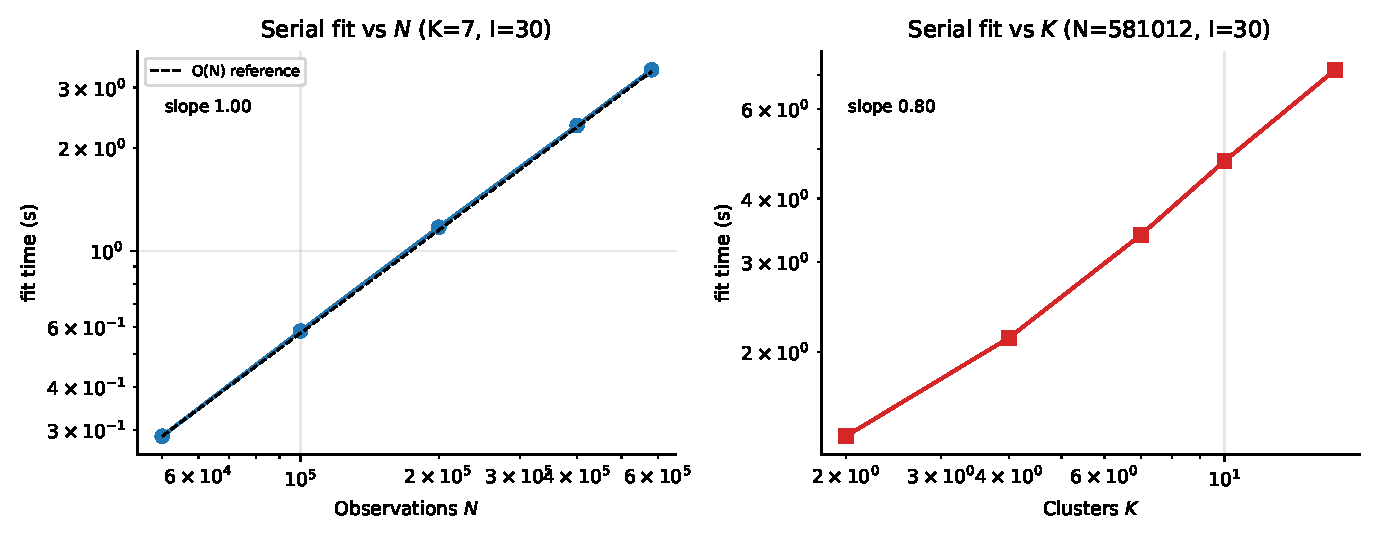
\includegraphics[width=\textwidth]{serial.pdf}
\caption{Serial fit scaling on Vanda. Left: N sweep at K=7; the reference line
is O(N). Right: K sweep at N=581,012. Three repetitions per point.}
\label{fig:serial}
\end{figure}

\section{MPI strong scaling}
\label{sec:strong}
\subsection{Four 64-core nodes}
Table~\ref{tab:strong} and Figure~\ref{fig:strong} show the primary strong
scaling result on four GN-A40 nodes. The one-rank MPI baseline is 2.887~s;
256 ranks reach 0.0223~s, a speedup of \textbf{129.7$\times$} and efficiency
\textbf{50.7\%}. Efficiency remains above 96\% through 16 ranks, then falls to
82.8\% (32 ranks), 78.3\% (64), 60.5\% (128) and 50.7\% (256). At 256 ranks
the per-rank workload is only 2,269 observations, and the two collectives
consume 9.7~ms, 43.7\% of the 22.3~ms fit. The local compute time is 13.3~ms;
the remainder is synchronization and imbalance. This is the expected transition
from computation-dominated to latency-dominated scaling for a small workload.

\begin{table}[H]
\centering\scriptsize
\caption{Vanda MPI strong scaling, N=581,012, K=7, D=54, I=30, 3 repetitions.
The first block is 4$\times$64 GN-A40; the second is 8$\times$32 CN.}
\label{tab:strong}
\resizebox{\textwidth}{!}{\begin{tabular}{llrrrrr}
\toprule
Layout & ranks & fit (s) & speedup & efficiency & collective (s) & collective share\\
\midrule
4$\times$64 & 1 & 2.8874 & 1.00 & 100.0\% & 0.0000 & 0.0\%\\
4$\times$64 & 2 & 1.4547 & 1.98 & 99.2\% & 0.0122 & 0.8\%\\
4$\times$64 & 4 & 0.7253 & 3.98 & 99.5\% & 0.0077 & 1.1\%\\
4$\times$64 & 8 & 0.3663 & 7.88 & 98.5\% & 0.0069 & 1.9\%\\
4$\times$64 & 16 & 0.1863 & 15.50 & 96.9\% & 0.0054 & 2.9\%\\
4$\times$64 & 32 & 0.1090 & 26.49 & 82.8\% & 0.0050 & 4.6\%\\
4$\times$64 & 64 & 0.0576 & 50.14 & 78.3\% & 0.0065 & 11.3\%\\
4$\times$64 & 128 & 0.0373 & 77.49 & 60.5\% & 0.0117 & 31.4\%\\
4$\times$64 & 256 & 0.0223 & 129.73 & 50.7\% & 0.0097 & 43.7\%\\
8$\times$32 & 1 & 2.8827 & 1.00 & 100.0\% & 0.0000 & 0.0\%\\
8$\times$32 & 2 & 1.4558 & 1.98 & 99.0\% & 0.0170 & 1.2\%\\
8$\times$32 & 4 & 1.0230 & 2.82 & 70.4\% & 0.3046 & 29.8\%\\
8$\times$32 & 8 & 0.5695 & 5.06 & 63.3\% & 0.2091 & 36.7\%\\
8$\times$32 & 16 & 0.2922 & 9.87 & 61.7\% & 0.1095 & 37.5\%\\
8$\times$32 & 32 & 0.1488 & 19.37 & 60.5\% & 0.0455 & 30.6\%\\
8$\times$32 & 64 & 0.0868 & 33.22 & 51.9\% & 0.0351 & 40.4\%\\
8$\times$32 & 128 & 0.4259 & 6.77 & 5.3\% & 0.3991 & 93.7\%\\
8$\times$32 & 256 & 0.4374 & 6.59 & 2.6\% & 0.4231 & 96.7\%\\
\bottomrule
\end{tabular}
}
\end{table}

\begin{figure}[H]
\centering
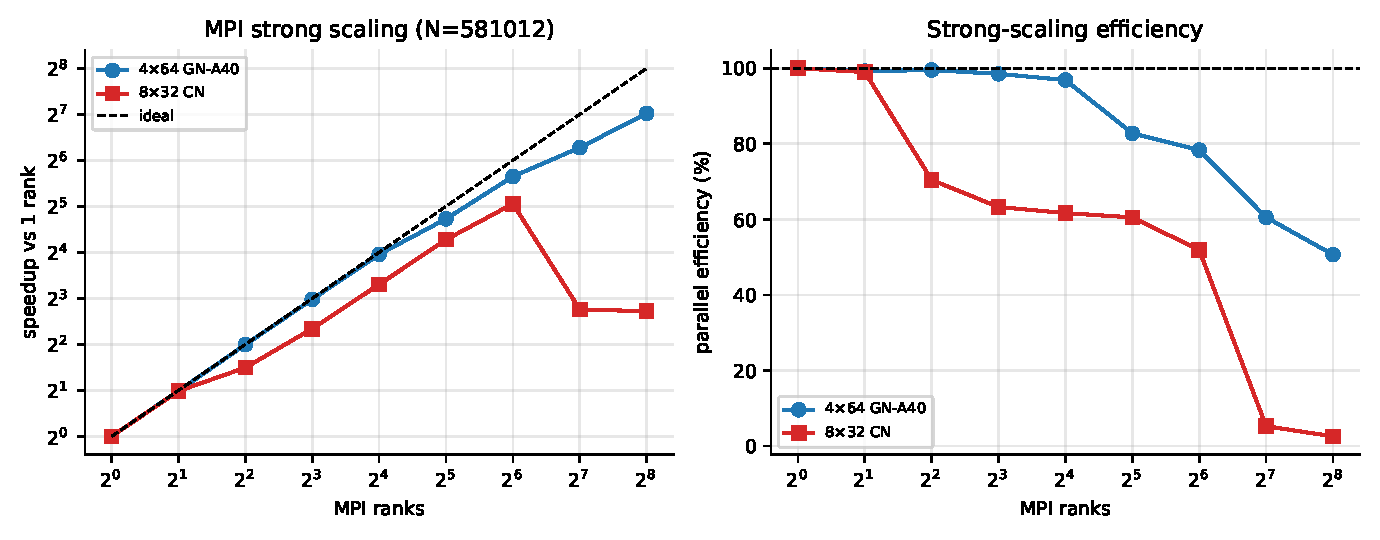
\includegraphics[width=\textwidth]{strong.pdf}
\caption{MPI strong scaling on Vanda. The 8$\times$32 curve is numerically
correct but its collective path collapses at 128--256 ranks; the two layouts
also differ in node family.}
\label{fig:strong}
\end{figure}

\subsection{Eight 32-core nodes and the topology anomaly}
The 8$\times$32 job uses the same CPU model string but a different node family
and node count. Its one-rank baseline is comparable (2.883~s), but from four
ranks onward the collective dominates: 0.305~s at 4 ranks, 0.399~s at 128 and
0.423~s at 256. Speedup collapses to 6.59$\times$ and efficiency to 2.6\% at
256 ranks. Crucially, \code{local\_compute\_s} at 256 ranks is 0.018~s in the
8$\times$32 job versus 0.013~s in the 4$\times$64 job: the arithmetic is not
the problem; the Allreduce is. The two jobs are not a clean 4-versus-8-node
experiment because GN-A40 and CN are different hardware families and the
placement of ranks differs. We therefore report the 8$\times$32 result as a
topology/placement observation, not as evidence that eight nodes are
inherently six times slower. The pinned-core experiment in
Section~\ref{sec:placement} shows that CN nodes can reach 0.0223~s at 256
ranks when placement is controlled.

The personal E2 campaign contains 24/27 rows: ranks 2--256 completed three repetitions each, while its one-rank run timed out at 300~s inside a mixed four-node allocation. Recovery job 1563234 isolated the singleton on one IN-010 node with binding disabled and completed three rows (median 3.429~s, hash \code{15912193932519828622}). This recovery is supplementary correctness/reproducibility evidence only: its Xeon Gold 6438N node differs from the GitHub four-node CN/GN campaign, so the primary 581k speedup curve remains the complete GitHub experiment.

\subsection{Independent fixed-total 10M strong scaling}
The personal Vanda extension evaluates the same deterministic logical 10-million-row workload at every rank count. This differs from weak scaling: total $N$ is fixed while local work shrinks as $P$ increases. The reported one-rank fit median is 49.805 s and the 256-rank median is 0.3744 s, giving approximately 133.0$\times$ speedup and 52.0\% efficiency. This is a separate campaign and is not merged into the GitHub 581k scaling curve.
\begin{figure}[H]\centering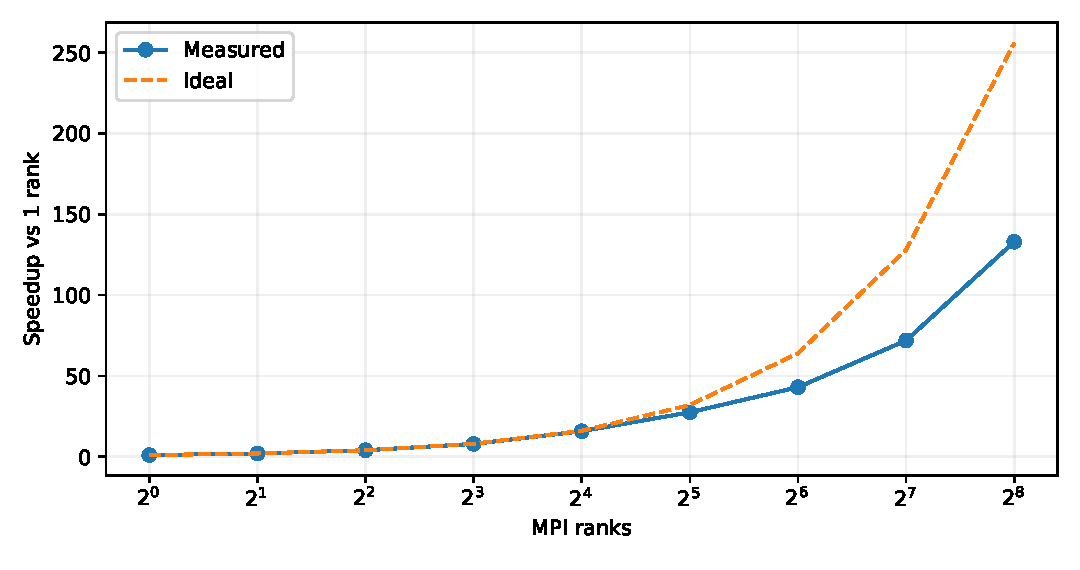
\includegraphics[width=.76\textwidth]{strong_10m.pdf}
\caption{Independent 10M fixed-total MPI strong-scaling speedup; ideal scaling shown for reference. Values are from the personal Vanda experiment and must not be interpreted as new independent forest records.}\label{fig:strong10m}\end{figure}
Increasing $N$ by about 17.2 times compared with original Covertype only modestly increases the reported 256-rank efficiency (50.7\% to 52.0\%). This comparison is descriptive across campaigns rather than a controlled same-allocation causal test; the communication-to-computation ratio alone does not explain all observed scaling losses.

\section{MPI weak scaling}
Figure~\ref{fig:weak} and Table~\ref{tab:weak} hold the per-rank workload at
50,000 observations while increasing the rank count from 1 to 256; the logical
dataset grows from 50,000 to 12.8 million. On 4$\times$64 the one-rank time is
0.3946~s and the 256-rank time is 0.4922~s, giving weak efficiency
\textbf{80.2\%}. Local compute is essentially constant (0.3945 to 0.4037~s);
the degradation is the collective, which rises from 0.00002~s to 0.2117~s at
256 ranks. On 8$\times$32 the same experiment reaches only \textbf{35.8\%}
because the collective is 0.827~s at 128 ranks and 0.813~s at 256. The
workload is balanced (50,000 observations every rank) and the label hashes
differ across rank counts by design, since each rank count defines a different
logical dataset. Weak efficiency therefore measures communication and
synchronization, not arithmetic imbalance.

\begin{table}[H]
\centering\scriptsize
\caption{Vanda MPI weak scaling, 50,000 observations per rank, K=7, D=54,
I=30, 3 repetitions.}
\label{tab:weak}
\resizebox{\textwidth}{!}{\begin{tabular}{llrrrrr}
\toprule
Layout & ranks & total $N$ & fit (s) & weak eff. & collective (s) & collective share\\
\midrule
4$\times$64 & 1 & 50,000 & 0.3946 & 100.0\% & 0.0000 & 0.0\%\\
4$\times$64 & 2 & 100,000 & 0.3975 & 99.3\% & 0.0039 & 1.0\%\\
4$\times$64 & 4 & 200,000 & 0.3995 & 98.8\% & 0.0084 & 2.1\%\\
4$\times$64 & 8 & 400,000 & 0.4021 & 98.1\% & 0.0092 & 2.3\%\\
4$\times$64 & 16 & 800,000 & 0.4024 & 98.1\% & 0.0109 & 2.7\%\\
4$\times$64 & 32 & 1,600,000 & 0.4062 & 97.1\% & 0.0131 & 3.2\%\\
4$\times$64 & 64 & 3,200,000 & 0.4151 & 95.1\% & 0.0212 & 5.1\%\\
4$\times$64 & 128 & 6,400,000 & 0.4827 & 81.8\% & 0.2019 & 41.8\%\\
4$\times$64 & 256 & 12,800,000 & 0.4922 & 80.2\% & 0.2117 & 43.0\%\\
8$\times$32 & 1 & 50,000 & 0.3916 & 100.0\% & 0.0000 & 0.0\%\\
8$\times$32 & 2 & 100,000 & 0.3976 & 98.5\% & 0.0035 & 0.9\%\\
8$\times$32 & 4 & 200,000 & 0.3969 & 98.6\% & 0.0080 & 2.0\%\\
8$\times$32 & 8 & 400,000 & 0.3979 & 98.4\% & 0.0085 & 2.1\%\\
8$\times$32 & 16 & 800,000 & 0.4010 & 97.6\% & 0.0146 & 3.6\%\\
8$\times$32 & 32 & 1,600,000 & 0.4047 & 96.8\% & 0.1243 & 30.7\%\\
8$\times$32 & 64 & 3,200,000 & 0.4564 & 85.8\% & 0.1755 & 38.4\%\\
8$\times$32 & 128 & 6,400,000 & 1.1078 & 35.3\% & 0.8270 & 74.7\%\\
8$\times$32 & 256 & 12,800,000 & 1.0946 & 35.8\% & 0.8132 & 74.3\%\\
\bottomrule
\end{tabular}
}
\end{table}

\begin{figure}[H]
\centering
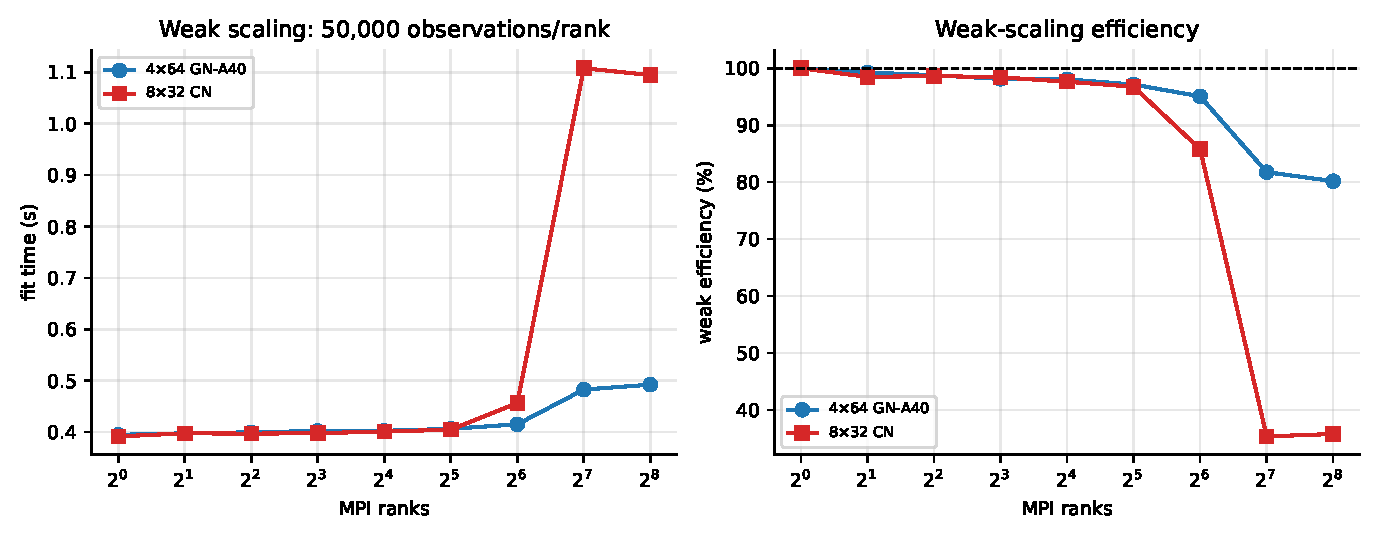
\includegraphics[width=\textwidth]{weak.pdf}
\caption{Weak scaling on Vanda. The 4$\times$64 layout retains 80.2\% at 256
ranks; the 8$\times$32 layout falls to 35.8\% because of collective latency.}
\label{fig:weak}
\end{figure}

\section{OpenMP scaling}
The independent Vanda extension supplies the missing one-node OpenMP-only sweep. Two workloads were tested using the same $K=7$, $D=54$, seed 42 and 30 fixed iterations: original Covertype ($581{,}012$ observations) and deterministic fixed-total 10M resampling. The one-thread and 64-thread median fit times are 2.5302 and 0.1045 seconds for the original data (24.2$\times$, 37.8\% efficiency), and 43.4167 and 1.7652 seconds for 10M (24.6$\times$, 38.4\%). These are within-workload speedups, not cross-machine comparisons. The growth in team size incurs synchronization, memory-bandwidth and scheduling costs; the measurements do not uniquely isolate those mechanisms.
\begin{table}[H]\centering\small
\caption{Independent Vanda OpenMP extension: fit-time medians in seconds. Each workload uses a separate one-thread baseline.}\label{tab:openmpvanda}
\begin{tabular}{rrrrr}\toprule
Threads & Original 581k & Speedup & Resampled 10M & Speedup\\\midrule
1&2.5302&1.00&43.4167&1.00\\
2&2.0053&1.26&30.8255&1.41\\
4&0.9795&2.58&16.8540&2.58\\
8&0.6203&4.08&8.9654&4.84\\
16&0.3707&6.83&4.7963&9.05\\
32&0.1967&12.87&3.0350&14.31\\
64&0.1045&24.21&1.7652&24.60\\\bottomrule
\end{tabular}\end{table}
\begin{figure}[H]\centering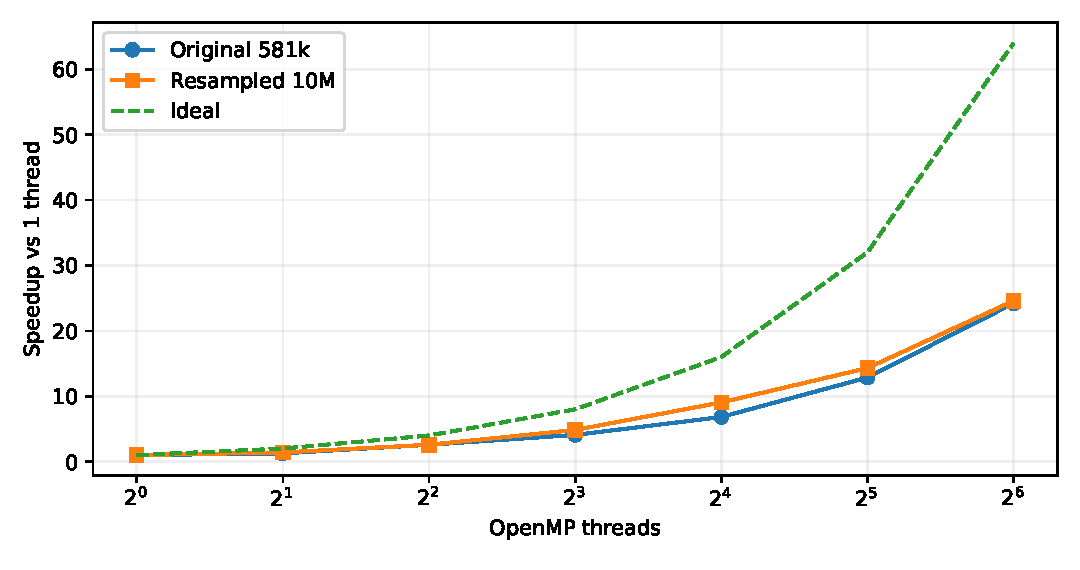
\includegraphics[width=.83\textwidth]{openmp_vanda.pdf}
\caption{Vanda OpenMP-only strong scaling within each workload. The two series use different dataset sizes and are compared by speedup, not absolute runtime.}\label{fig:openmpvanda}\end{figure}
For platform context, the GitHub baseline also includes a smaller Apple M1 Pro OpenMP thread sweep, shown below. It is not combined with the Vanda curve.

\begin{table}[H]
\centering\small
\caption{Measured OpenMP scaling on Apple M1 Pro, one MPI rank, N=581,012,
K=7, I=30, median of 3.}
\label{tab:openmp}
\begin{tabular}{rrrrr}
\toprule
threads & fit (s) & speedup & efficiency & thread reduction (s)\\
\midrule
1 & 4.2708 & 1.00 & 100.0\% & 1.30e-05\\
2 & 2.2583 & 1.89 & 94.6\% & 1.20e-05\\
4 & 1.1852 & 3.60 & 90.1\% & 2.90e-05\\
\bottomrule
\end{tabular}

\end{table}

\begin{figure}[H]
\centering
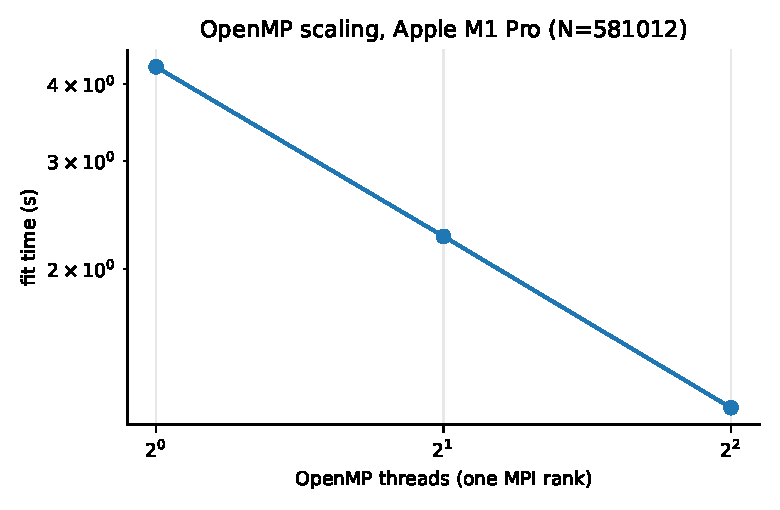
\includegraphics[width=0.62\textwidth]{openmp.pdf}
\caption{OpenMP-only fit time on the M1 Pro. Only 1, 2 and 4 threads were
measured in the committed baseline; this is not a Vanda curve.}
\label{fig:openmp}
\end{figure}

\section{Hybrid MPI+OpenMP}
\label{sec:hybrid}
\subsection{Equal 64-core budgets}
Table~\ref{tab:hybrid64} and Figure~\ref{fig:hybrid64} compare seven layouts
whose ranks $\times$ threads product is exactly 64, on one 64-core IN node.
The MPI-only 64$\times$1 layout is fastest at 0.0779~s. All multi-thread
layouts are slower: 32$\times$2 is 0.0833~s (0.94$\times$ the MPI-only
baseline), 16$\times$4 and 8$\times$8 are 0.0859/0.0856~s, 2$\times$32 is
0.0872~s, and 1$\times$64 is 0.1020~s (0.76$\times$). The phase breakdown
explains why:
\begin{itemize}
\item MPI collective time falls from 0.0259~s at 64$\times$1 to 0.00002~s at
      1$\times$64, as expected when the number of ranks collapses;
\item local compute rises from 0.0736~s to 0.1011~s, because a 64-thread team
      has more synchronization and less efficient per-thread streaming than 64
      independent single-threaded ranks;
\item the explicit OpenMP fold is cheap, rising from 0.000013~s to
      0.000526~s; it is not the dominant cost.
\end{itemize}
The result is a genuine trade-off, not a failure of Hybrid: fewer ranks reduce
collective traffic, but the OpenMP team loses more in local execution than it
saves in communication at this problem size. Hybrid is therefore not assumed
to outperform MPI-only.

\begin{table}[H]
\centering\small
\caption{Hybrid layouts at a fixed 64-core budget, one Vanda IN node,
N=581,012, K=7, D=54, I=30, 3 repetitions. Speedup is relative to
64$\times$1.}
\label{tab:hybrid64}
\resizebox{\textwidth}{!}{\begin{tabular}{rrrrrrr}
\toprule
ranks & threads & fit (s) & speedup vs 64$\times$1 & local (s) & collective (s) & thread reduction (s)\\
\midrule
64 & 1 & 0.0779 & 1.00 & 0.0736 & 0.02590 & 1.30e-05\\
32 & 2 & 0.0833 & 0.94 & 0.0811 & 0.00955 & 2.50e-05\\
16 & 4 & 0.0859 & 0.91 & 0.0831 & 0.00986 & 3.60e-05\\
8 & 8 & 0.0856 & 0.91 & 0.0840 & 0.00613 & 6.00e-05\\
4 & 16 & 0.0853 & 0.91 & 0.0840 & 0.00362 & 1.11e-04\\
2 & 32 & 0.0872 & 0.89 & 0.0865 & 0.00301 & 2.09e-04\\
1 & 64 & 0.1020 & 0.76 & 0.1011 & 0.00002 & 5.26e-04\\
\bottomrule
\end{tabular}
}
\end{table}

\begin{figure}[H]
\centering
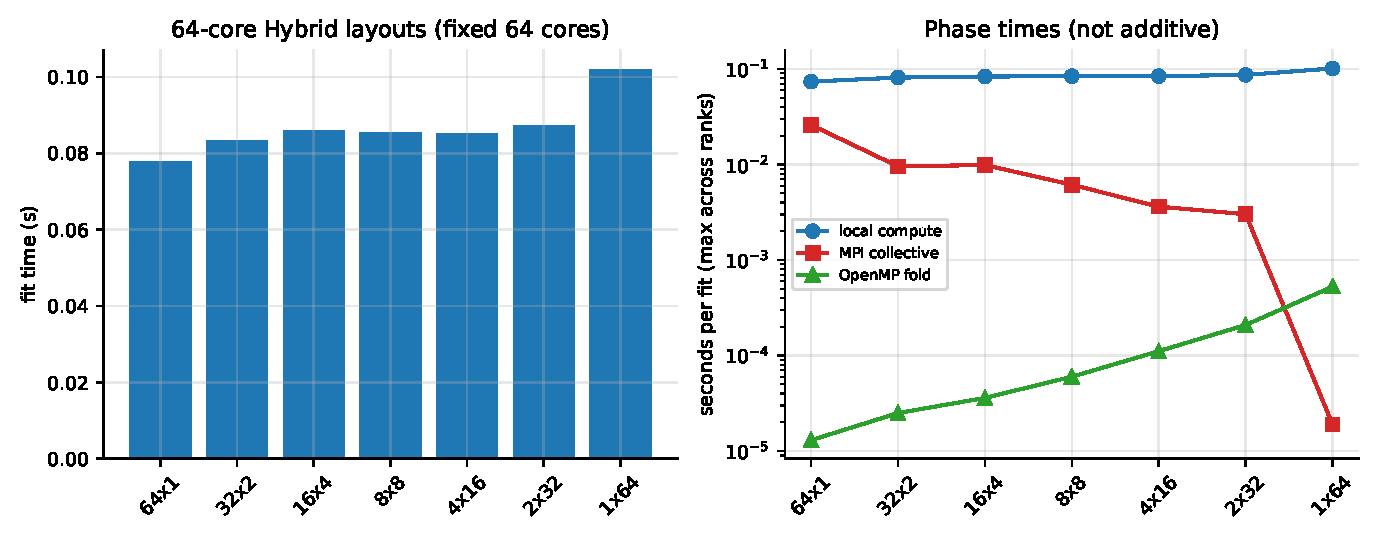
\includegraphics[width=\textwidth]{hybrid64.pdf}
\caption{Left: fit time for seven equal-64-core Hybrid layouts. Right:
phase times; these are maxima across ranks and are not additive, so they are
plotted as separate series rather than stacked.}
\label{fig:hybrid64}
\end{figure}

\subsection{256 cores: invalid unpinned runs and the pinned rerun}
\label{sec:placement}
The committed 256-core unpinned Hybrid CSVs are internally inconsistent and
must not be used as performance evidence. For layout 256$\times$1 the three
repetitions are 0.0273, 0.7690 and 1.0875~s, a 40$\times$ spread; the other
layouts are around 1.3--3.0~s, and the measured collective reaches 2.0~s. The
8$\times$32 variant shows the same pattern (0.0365, 0.7746, 0.8044~s for
256$\times$1; 3.4--4.1~s for 8$\times$32). These rows are retained for
diagnosis but excluded from all conclusions.

The later pinned-core experiment reruns only the legal pinned layout,
256$\times$1, on four 64-core CN nodes with \code{--map-by core --bind-to core}
and five repetitions. It gives 0.02208--0.02410~s, median \textbf{0.02227~s},
standard deviation 0.00083~s (CV 3.7\%), and the same label hash as the MPI
runs. This is statistically indistinguishable from the MPI-only 256-rank
4$\times$64 result (0.02226~s) and from the fastest unpinned repetition, while
removing the 40$\times$ variability. This is consistent with a
placement/binding contribution, but the pinned run also changed the job
allocation and environment; the experiment does not isolate affinity as the
sole cause. It does show that CN nodes can deliver 0.022~s at 256 ranks under
controlled placement, so the 8$\times$32 anomaly is not a simple ``CN hardware
is slow'' effect.

\begin{table}[H]
\centering\small
\caption{256-core Hybrid 256$\times$1: MPI-only baseline, pinned rerun and
invalid unpinned run. `--' marks a value not available from the three-rep
summary.}
\label{tab:hybrid256}
\begin{tabular}{lrrrrrr}
\toprule
Configuration & reps & median (s) & min (s) & max (s) & SD (s) & collective (s)\\
\midrule
MPI-only 256 ranks & 3 & 0.0223 & 0.0214 & 0.0281 & -- & 0.0097\\
Hybrid 256$\times$1 pinned & 5 & 0.0223 & 0.0221 & 0.0241 & 0.0008 & 0.0106\\
Hybrid 256$\times$1 unpinned & 3 & 0.7690 & 0.0273 & 1.0875 & 0.5440 & 0.7558\\
\bottomrule
\end{tabular}

\end{table}

\begin{figure}[H]
\centering
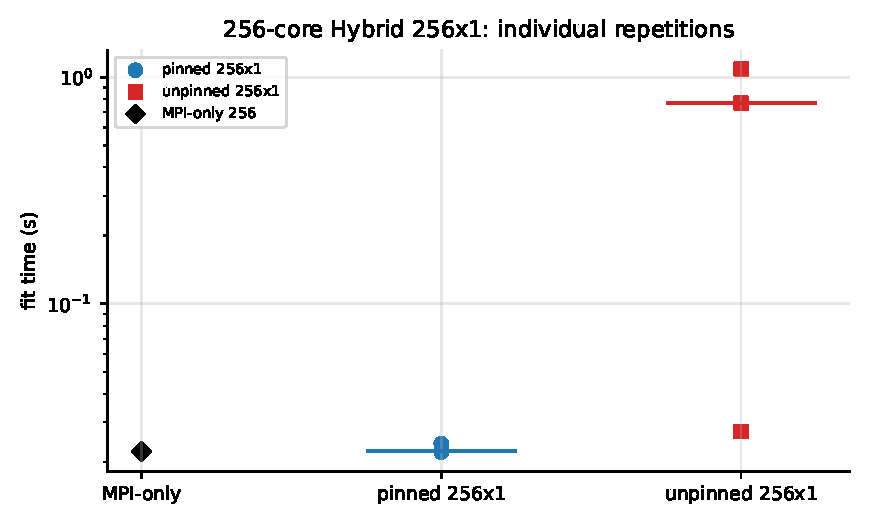
\includegraphics[width=0.66\textwidth]{hybrid256.pdf}
\caption{The pinned 256$\times$1 Hybrid run is stable and matches the MPI-only
fit; the unpinned run spans a 40$\times$ range. Log scale.}
\label{fig:hybrid256}
\end{figure}

The pinned experiment does not validate multi-thread layouts with real
per-rank core reservation: the available launcher hangs for \code{pe=} forms,
and \code{--bind-to core} would pin a whole OpenMP team to one core. The only
correctly pinned Hybrid layout is therefore 256$\times$1, which is effectively
MPI-only. This is a limitation of the placement study, not a reason to treat
the invalid multi-thread rows as valid.

\subsection{Independent 10M hybrid experiments and incomplete configurations}
The personal Vanda extension runs deterministic 10M resampling at fixed worker budgets. At 64 workers the seven layout medians (64$\times$1 through 1$\times$64) are 1.2568, 1.5102, 1.4241, 1.4040, 1.5800, 1.5539 and 1.7348 seconds, respectively. MPI-only 64$\times$1 is again fastest within this campaign, although one of its repetitions was unusually slow (2.3895 s), warranting a variability caveat. The original GitHub 581k 64-worker comparison remains a distinct experiment, not an additional replicate.

At 256 workers, six unpinned multithreaded layouts completed three repetitions each. The 256$\times$1 layout failed its original preflight, but an independent recovery (job 1563235, four CN nodes) completed three pinned-core repetitions at a median of \textbf{0.32014~s}, with label hash \code{14076111245358280480} and SSE 64,089,789.818295. The recovery ran with \code{--map-by core --bind-to core}, whereas the six multi-thread layouts used unbound placement; it is a separate PBS allocation. Table~\ref{tab:e6_256_recovery} and Figure~\ref{fig:e6_256_recovery} therefore report seven measured configurations with the binding/allocation distinction explicit.

The recovered 256$\times$1 time is lower than the six unpinned multi-thread layouts in this campaign (0.489--0.599~s), but this is not a controlled test that MPI-only is inherently faster: binding policy, node allocation and rank/thread topology all change together. The 10M MPI-only 256-rank median from the separate E3 job (0.3744~s) is a contextual reference, not a same-allocation baseline.

\begin{table}[H]
\centering\small
\caption{Personal Vanda 10M Hybrid at 256 workers. The first six rows are the unpinned original campaign; the last row is the separate pinned 256$\times$1 recovery. Medians of three repetitions.}
\label{tab:e6_256_recovery}
\begin{tabular}{rrrlrr}
\toprule
ranks & threads & workers & binding/allocation & median fit (s) & reps\\
\midrule
128 & 2 & 256 & unpinned; original 4$\times$64 & 0.4972 & 3\\
64 & 4 & 256 & unpinned; original 4$\times$64 & 0.4891 & 3\\
32 & 8 & 256 & unpinned; original 4$\times$64 & 0.5121 & 3\\
16 & 16 & 256 & unpinned; original 4$\times$64 & 0.5347 & 3\\
8 & 32 & 256 & unpinned; original 4$\times$64 & 0.5584 & 3\\
4 & 64 & 256 & unpinned; original 4$\times$64 & 0.5994 & 3\\
256 & 1 & 256 & pinned core; separate 4$\times$CN & 0.3201 & 3\\
\bottomrule
\end{tabular}

\end{table}

\begin{figure}[H]
\centering
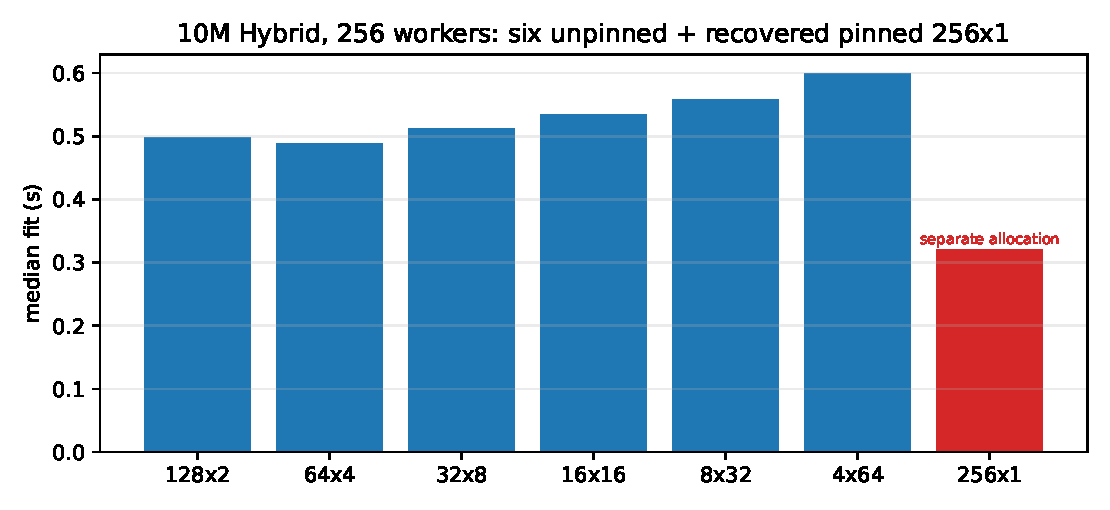
\includegraphics[width=.82\textwidth]{e6_256_recovery.pdf}
\caption{Measured 10M Hybrid configurations at 256 workers. The red bar is the separately allocated pinned 256$\times$1 recovery; the blue bars are the unpinned original campaign.}
\label{fig:e6_256_recovery}
\end{figure}

The original 128-worker job 1557221, backup smoke 1563236 and dependent backup 1563237 were still queued/held at the final bounded status check; no 128-worker timing is claimed. The personal 581k MPI campaign has 24/27 rows because its one-rank run failed; recovery 1563234 supplies that missing point only as supplementary evidence, as explained in Section~\ref{sec:strong}.

\section{GPU evaluation}
\subsection{NVIDIA CUDA on Vanda}
Table~\ref{tab:cuda} and Figure~\ref{fig:cuda} summarize 30 runs on one A40.
At N=581,012 the assignment kernel takes 0.365~ms, the CPU double-precision
assignment pass takes 89.5~ms, and the full Stage-B fit takes 0.644~s. The
kernel is much faster than the CPU assignment, but the end-to-end fit is
dominated by CPU accumulation (0.613~s) and label readback (0.007~s), not by
the kernel. Stage~A is slower (2.109~s full fit) because it re-uploads the
observation matrix every iteration: 1.492~s of upload time at 581,012. The
Stage-B optimization, keeping the matrix resident, reduces the full fit by
about 3.3$\times$ at the largest size.

Numerical agreement is exact for 50k, 100k, 200k and 581k; at 400k it is
0.9999875 with maximum centroid difference $8.54\times10^{-5}$ and relative
inertia difference $3.2\times10^{-8}$. This is consistent with float32 device
arithmetic against a float64 host reference and is not a correctness failure.
The comparison in the figure is assignment-to-assignment and fit-to-fit; the
0.365~ms kernel time is never presented as a 245$\times$ end-to-end speedup.
The GPU still performs only the assignment; accumulation and centroid update
remain on the CPU, which is the main optimization opportunity.

\begin{table}[H]
\centering\scriptsize
\caption{CUDA A40 medians, 3 repetitions per point. Kernel is CUDA-event
time in milliseconds; all other times are seconds. Agreement is against the
in-process double-precision CPU reference.}
\label{tab:cuda}
\resizebox{\textwidth}{!}{\begin{tabular}{llrrrrrrr}
\toprule
stage & $N$ & fit (s) & kernel (ms) & CPU assign (s) & upload (s) & readback (s) & accumulate (s) & agreement\\
\midrule
A\_assign & 50,000 & 0.0964 & 0.035 & 0.0080 & 0.0706 & 0.0009 & 0.0271 & 1.000000\\
A\_assign & 100,000 & 0.2354 & 0.072 & 0.0162 & 0.1628 & 0.0017 & 0.0742 & 1.000000\\
A\_assign & 200,000 & 0.6939 & 0.132 & 0.0324 & 0.4906 & 0.0030 & 0.2023 & 1.000000\\
A\_assign & 400,000 & 1.4238 & 0.253 & 0.0635 & 1.0025 & 0.0056 & 0.4262 & 0.999988\\
A\_assign & 581,012 & 2.1088 & 0.362 & 0.0895 & 1.4923 & 0.0076 & 0.6218 & 1.000000\\
B\_full & 50,000 & 0.0301 & 0.035 & 0.0081 & 0.0046 & 0.0012 & 0.0270 & 1.000000\\
B\_full & 100,000 & 0.0600 & 0.071 & 0.0162 & 0.0083 & 0.0021 & 0.0541 & 1.000000\\
B\_full & 200,000 & 0.1851 & 0.132 & 0.0324 & 0.0175 & 0.0039 & 0.1723 & 1.000000\\
B\_full & 400,000 & 0.4326 & 0.252 & 0.0633 & 0.0336 & 0.0056 & 0.4104 & 0.999988\\
B\_full & 581,012 & 0.6444 & 0.365 & 0.0895 & 0.0495 & 0.0070 & 0.6129 & 1.000000\\
\bottomrule
\end{tabular}
}
\end{table}

\begin{figure}[H]
\centering
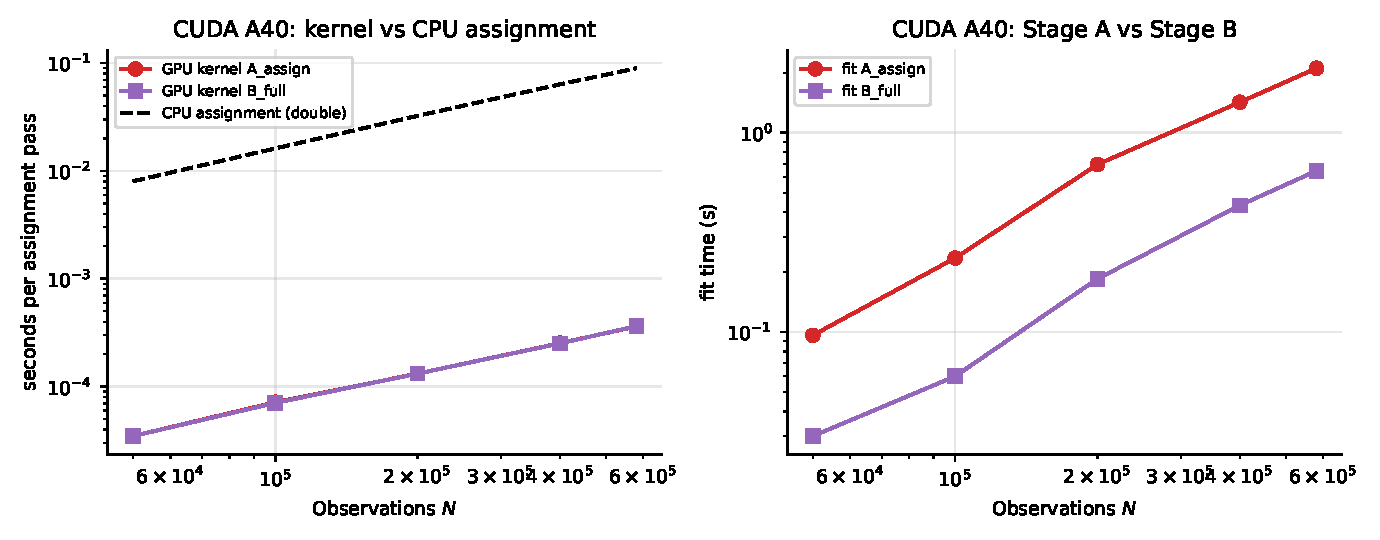
\includegraphics[width=\textwidth]{cuda.pdf}
\caption{CUDA A40. Left: assignment kernel versus a CPU double-precision
assignment pass. Right: full Stage-A and Stage-B fit times. Kernel time is not
compared with CPU end-to-end time.}
\label{fig:cuda}
\end{figure}

\subsection{Apple Metal (separate platform)}
The Metal implementation on an M1 Pro agrees with the CPU labels at every
measured size (20k--400k) and has label agreement 1.0. At 400k the Stage-A fit
is 0.915~s, Stage-B is 0.673~s, the GPU kernel is 0.020~s and the CPU
assignment is 0.079~s. The same caveat applies: the kernel is faster than the
CPU assignment, but neither GPU stage beats the best CPU implementation
end-to-end, and the hardware is not Vanda. Metal is reported only as a
secondary GPU portability result.

\begin{figure}[H]
\centering
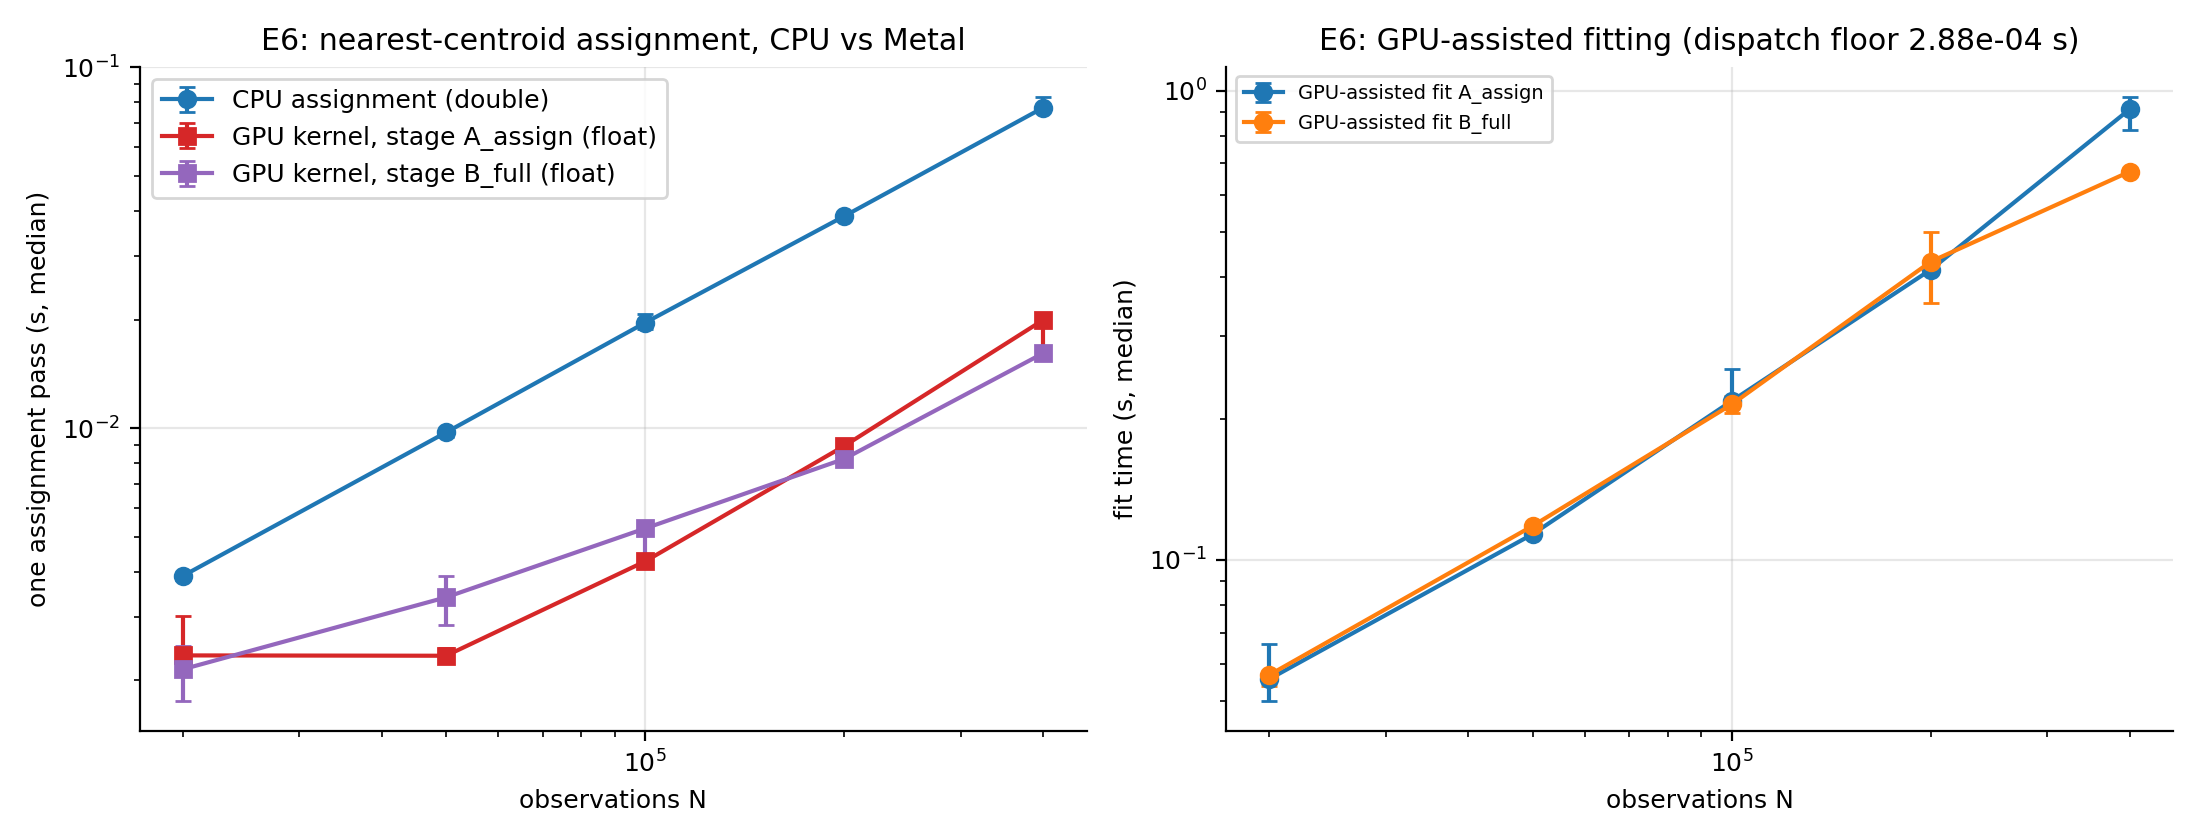
\includegraphics[width=0.92\textwidth]{metal.png}
\caption{Apple Metal evaluation on an M1 Pro. This is a separate platform
from the Vanda CPU/CUDA results and is not mixed into a scaling curve.}
\label{fig:metal}
\end{figure}

\section{Communication, affinity and additional experiments}
Figure~\ref{fig:comm} isolates the collective behaviour. On 4$\times$64 the
Allreduce is 5--12~ms and its share is below 5\% until 64 ranks, then rises to
31\% at 128 and 44\% at 256. On 8$\times$32 the collective is already 30\% at
four ranks, 94\% at 128 and 97\% at 256. The K-means payload is only 3,088
bytes per rank per iteration, so this is latency and placement, not bandwidth.
The timing includes waiting for slower ranks; it is not pure network transfer.

\begin{figure}[H]
\centering
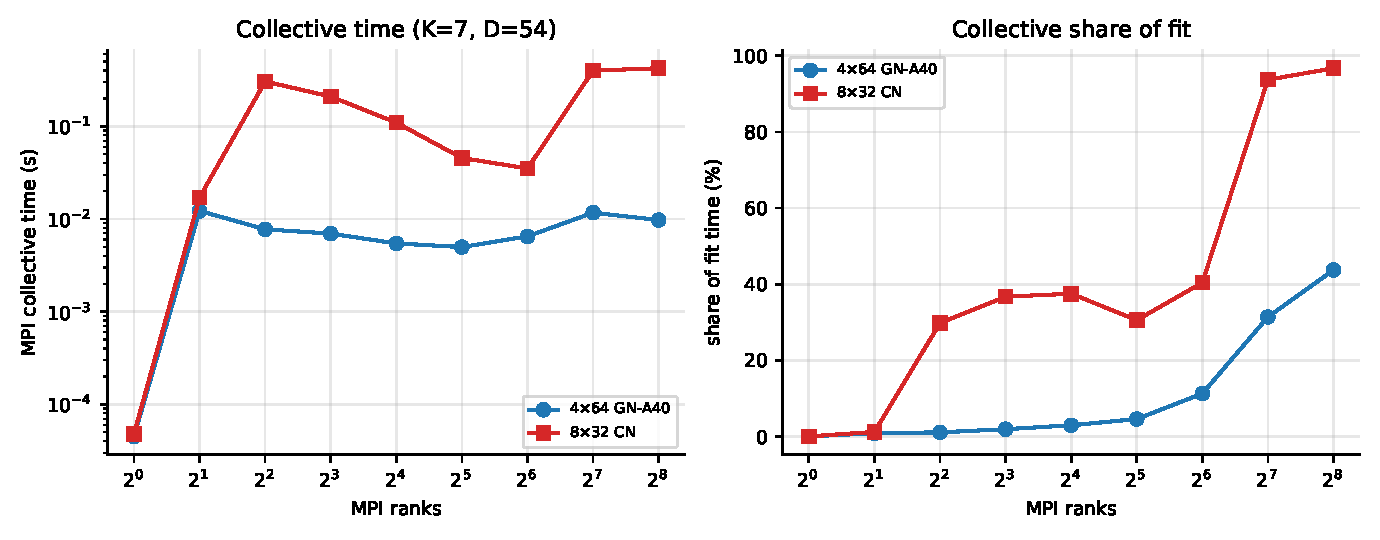
\includegraphics[width=\textwidth]{communication.pdf}
\caption{MPI collective time and its share of fit. The 8$\times$32 anomaly is
a topology/placement observation; the 4$\times$64 and 8$\times$32 jobs also
use different node families.}
\label{fig:comm}
\end{figure}

\paragraph{Pinned-core experiment.}
The latest measured additional experiment is the five-repetition pinned
256$\times$1 Hybrid run described in Section~\ref{sec:placement}. Its research
question is explicit in the committed script: the unpinned 256$\times$1 fit
varied from 0.027 to 1.088~s, while the pinned K-means phase timers were small
and stable. The corrected run pins every rank to a core on four 64-core CN
nodes and produces 0.0221--0.0241~s, CV 3.7\%. This supports the placement
explanation, but it does not prove which of binding, NUMA placement or
competing OpenMP threads caused the unpinned values; the experiment controls
binding only and uses one thread per rank.

\paragraph{Allreduce microbenchmark (incomplete).}
\path{tests/allreduce_micro.cpp} and \path{jobs/vanda/allreduce_probe.pbs}
are committed to isolate the exact 3,088-byte payload with pinned/unpinned
ranks and competing OpenMP threads. Their research question is the right one,
but \textbf{no output CSV or log is committed}. The probe is therefore
classified INCOMPLETE/UNVERIFIED and no Allreduce-microbenchmark number is
reported. The K-means phase timers remain the measured communication evidence.

\subsection{Independent eight-node placement study}
The personal E7 experiment produced 10/10 expected records on eight nodes. For 128 ranks, mean fit times were 0.1509 s (core mapping), 0.3323 s (PPR16), and 0.1684 s (PPR32). For 256 ranks, the corresponding available means were 0.5262 s (core) and 0.4800 s (PPR32). Collective-phase times closely tracked these differences; all runs reported the same original-data label hash and SSE. Only two repetitions were available per configuration, so these observations support placement sensitivity, not a statistically definitive ranking or a pure network-latency explanation. The GitHub pinned 256$\times$1 experiment also shows reduced variability, but different job conditions prevent attributing the entire improvement solely to affinity.

\section{Correctness validation}
The repository's test suite compares serial, OpenMP, MPI and Hybrid results on
a synthetic mixture, real Covertype, K=1 and K=7, uneven partitions, more ranks
than observations, fixed-iteration and convergence stopping, and the
empty-cluster policy. The measured performance files provide independent
cross-rank evidence:
\begin{itemize}
\item E2 4$\times$64: every rank count from 1 to 256 produces the same label
      hash \code{15912193932519828622}; the scaling difference is therefore not
      a different clustering.
\item E2 8$\times$32: the same single hash, so its anomaly is communication,
      not numerical divergence.
\item E4 64-core: all seven layouts share one hash; the pinned 256$\times$1
      run also has that hash.
\item CUDA: label agreement 1.0 for all but 400k (0.9999875), maximum centroid
      difference $8.54\times10^{-5}$ and relative inertia difference
      $3.2\times10^{-8}$; Metal agreement is 1.0.
\end{itemize}
Floating-point reductions are not required to be bitwise equal: sums over
different rank/thread orders differ in the last bits. The acceptance criterion
is exact label/cluster-size agreement and tolerance-based centroid/inertia
agreement, with any differing clustering treated as a failure to explain.

The original-data convergence run used for Section~\ref{sec:realdata} ran 91
iterations and converged. It is an analysis run from the GitHub baseline
serial binary and data, not a personal HPC result and not a fixed-iteration
benchmark.

\section{Real-data Covertype interpretation}
\label{sec:realdata}
The performance workloads are resampled and must not be interpreted as new
forest records. For the real-data interpretation we use only the original
581,012 observations. A converged serial run (91 iterations) gives inertia
\textbf{3,712,497.96} and the cluster sizes in Table~\ref{tab:covertype}.
Against the seven known cover types, \textbf{ARI = 0.0220}, \textbf{NMI =
0.0650} and \textbf{AMI = 0.0649}.

\begin{table}[H]
\centering\small
\caption{Converged original-Covertype clusters. Elevation, road distance and
fire distance are inverse-transformed means in the original units.}
\label{tab:covertype}
\resizebox{\textwidth}{!}{\begin{tabular}{rrrrrrrr}
\toprule
cluster & size & share & majority type & purity & elevation & road dist. & fire dist.\\
\midrule
0 & 77,764 & 13.4\% & 1 & 0.500 & 3110 & 4352 & 2103\\
1 & 56,307 & 9.7\% & 2 & 0.445 & 3179 & 2217 & 1880\\
2 & 50,440 & 8.7\% & 2 & 0.404 & 2680 & 1477 & 1287\\
3 & 51,673 & 8.9\% & 2 & 0.712 & 2925 & 3764 & 5070\\
4 & 125,172 & 21.5\% & 1 & 0.462 & 3053 & 2472 & 1560\\
5 & 66,197 & 11.4\% & 2 & 0.411 & 2793 & 1485 & 1473\\
6 & 153,459 & 26.4\% & 2 & 0.538 & 2901 & 1469 & 1704\\
\bottomrule
\end{tabular}
}
\end{table}

\begin{figure}[H]
\centering
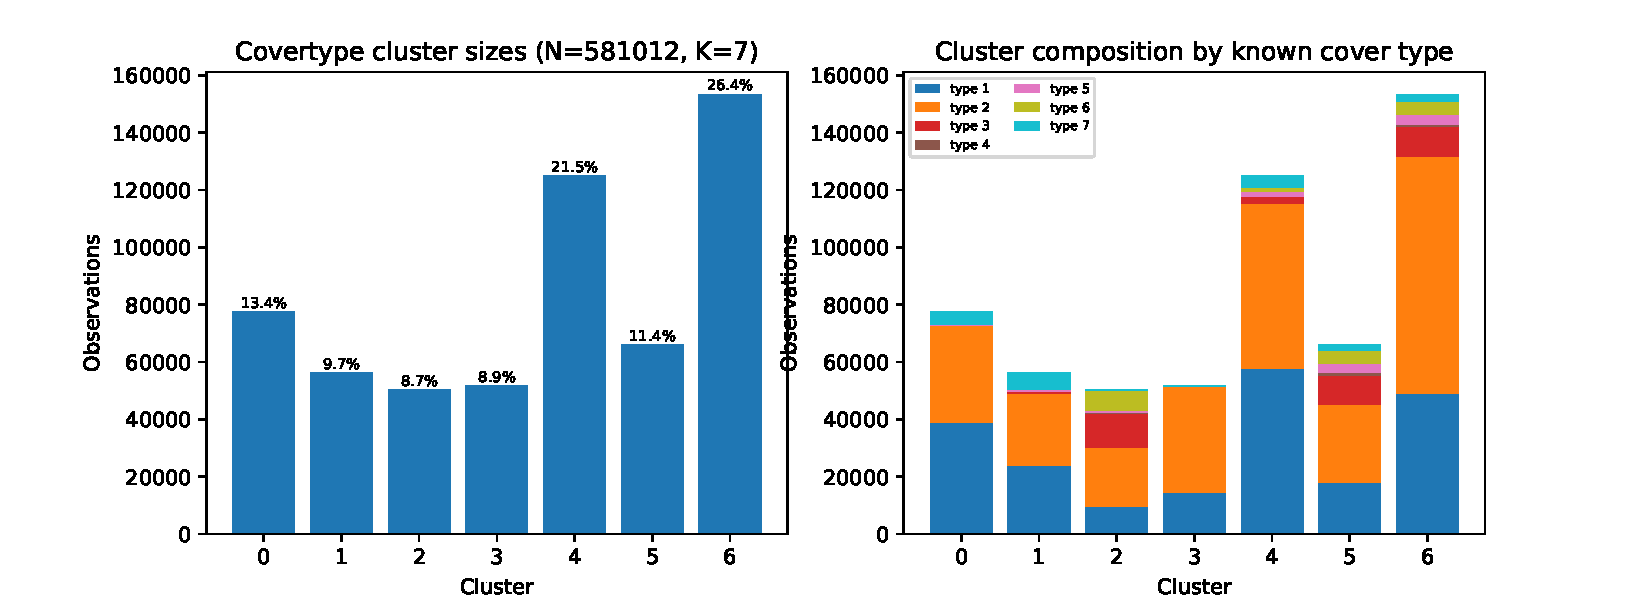
\includegraphics[width=\textwidth]{covertype_clusters.pdf}
\caption{Real-data Covertype cluster sizes and cover-type composition, K=7,
original 581,012 observations. This is separate from all resampled performance
data.}
\label{fig:covertype}
\end{figure}

\begin{figure}[H]
\centering
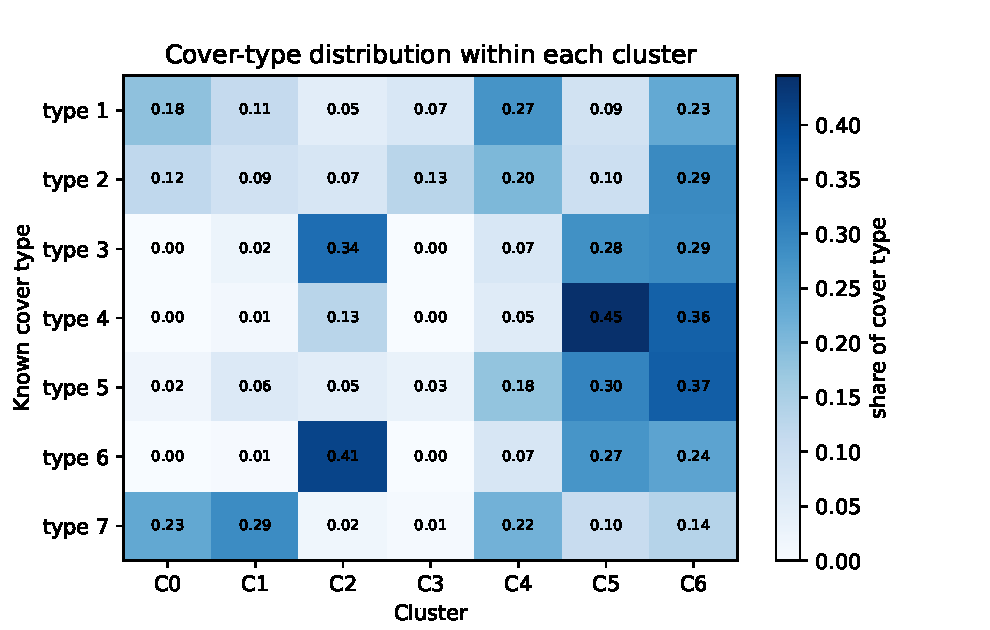
\includegraphics[width=0.72\textwidth]{covertype_contingency.pdf}
\caption{Row-normalized cover-type distribution within each cluster.}
\label{fig:covertype-cont}
\end{figure}

The clusters are not the seven cover types. Every cluster is a mixture,
and the two dominant classes (Lodgepole Pine, 283,301 observations, and
Spruce/Fir, 211,840) occupy most of every cluster. Cluster~3 is the purest
(71.2\% type 2), with the largest mean fire distance (5,070) and a high
elevation (2,925); cluster~0 is 50.0\% type 1 with a large mean road distance
(4,352); clusters~2 and~5 are lower-elevation, steeper-slope groups with more
type 3/6 observations; cluster~4 is the largest (125,172) and 46.2\% type 1.
Rare types are split rather than recovered: 45\% of type-4 observations fall
in cluster~5 and 34\% of type-3 observations fall in cluster~2, but those
clusters remain majority types 1/2.

The low ARI/NMI has a clear explanation. Euclidean K-means on ten standardized
continuous features plus 44 binary indicators is dominated by the high-variance
continuous dimensions and by the binary soil/wilderness patterns; the binary
features are not weighted, and the class imbalance lets the two large classes
dominate the centroid means. K=7 is a modelling choice matching the number of
labels, not a guarantee that the label geometry is seven well-separated
Euclidean clusters. This is a real-data conclusion about the clustering, not a
performance claim, and no resampled workload enters it.

\section{Discussion and limitations}
\paragraph{Why efficiency falls.}
Amdahl's argument \citep{amdahl1967} and its scaled counterpart \citep{gustafson1988} frame the expected limit: at fixed N, increasing P reduces per-rank work while the two collectives remain
per-iteration barriers. On the 581k workload, 256 ranks hold only 2,269
observations each; the 3 KB Allreduce is latency-bound and consumes 44\% of
the fit on the good layout. The 10M-equivalent weak workload keeps 50,000
observations/rank and retains 80.2\% on 4$\times$64, showing that a larger
per-rank workload amortizes the collective. This is the expected
compute-to-communication trade-off, not a defect in the algorithm.

\paragraph{Node layout versus hardware.}
The 4$\times$64 and 8$\times$32 campaigns are not a controlled node-count
experiment: GN-A40 and CN are different node families, and the 8$\times$32
collective collapses by an order of magnitude while local compute stays
similar. The correct conclusion is that the 8$\times$32 configuration in this
campaign suffered a collective/placement problem. The pinned 256$\times$1 run
on four CN nodes reaches the MPI-only time, showing that the CN hardware can
perform well under binding; it does not isolate node count from fabric.

\paragraph{Hybrid trade-offs.}
At 64 cores, MPI-only 64$\times$1 is 24\% faster than 1$\times$64 (0.0779 vs
0.1020~s). The collective share falls as the rank count falls, but local
compute becomes slower with large OpenMP teams; the explicit fold is cheap
(0.5~ms at 64 threads), so the loss is not the fold alone. Hybrid should be
selected only when the communication saving outweighs the OpenMP scheduling
cost, and only with verified affinity. The pinned 256$\times$1 result is
effectively MPI-only and should not be presented as evidence that multi-thread
Hybrid scales.

\paragraph{GPU trade-offs.}
The A40 kernel is far faster than the CPU assignment, but Stage-B still spends
0.613~s in CPU accumulation and 0.007~s in readback at 581k, versus 0.365~ms
in the kernel. A GPU-resident accumulation/centroid update, or a fused
reduction, is the obvious next step. A kernel-only comparison would be
misleading and is deliberately avoided.

\paragraph{Limitations.}
(i) The personal Vanda OpenMP sweep supplements the baseline, but uses a separate allocation and source version. (ii) The baseline unpinned 256-core Hybrid rows are invalid; the personal 10M set contains six unpinned layouts plus a separately allocated pinned 256$\times$1 recovery, so it is not a same-allocation binding control. (iii) The Allreduce microbenchmark was committed without results. (iv) The 4$\times$64 and 8$\times$32 layouts are hardware-confounded. (v) GPU results use one A40 and float32 device arithmetic; Metal is a different platform. (vi) The real-data analysis is a deterministic single-seed K-means result, not a statistical guarantee over initializations. (vii) The GitHub serial sweep covers $N\le581{,}012$; the personal 1M/5M/10M points use fixed-total resampled logical rows. (viii) E6-128 remains queued (1557221), its backup smoke 1563236 is queued and production 1563237 is held; no 128-worker timing is claimed. (ix) The E2 one-rank recovery 1563234 is supplementary because its IN-010 node differs from the primary 4$\times$64 allocation.

\section{Practical Challenges of Large-Scale HPC Experimentation}

The scaling results above are measurements of both the algorithm and the
execution environment. Vanda is a shared PBS cluster, and a request for 256
CPU cores is a request for a particular combination of nodes, cores, memory
and topology, not a guarantee of immediate access to 256 interchangeable
cores. This section records the operational evidence behind the incomplete
and heterogeneous configurations, and separates it from the K-means scaling
conclusions.

\subsection{Resource contention and queueing delays}
Large jobs were scheduled only when a suitable multi-node shape was free.
The original E6-128 job 1557221 requested two 64-core nodes and was still
queued at the final status check, more than 46 hours after its creation; its
scheduler comment was \code{Insufficient amount of resource: node\_pool}. The
E6-128 backup smoke 1563236 requested the same 2$\times$64 shape and was still
queued after about 22 hours, with the same comment. The 256$\times$1 recovery
1563235 was created on 16 November at 13:48 and started on 17 November at
04:30, an observed queue wait of about 14 h 42 min, for only 18 seconds of
execution. By contrast, the one-core E2 recovery 1563234 started after about
8 seconds. These waits are scheduler observations from \code{ctime} and
\code{stime}, not estimates.

Resource fragmentation matters: a 4$\times$64 request can wait even when the
cluster has 256 free cores in aggregate, because the scheduler must satisfy a
node-count, per-node-core and memory shape simultaneously. Queue policy,
competing users and heterogeneous node families add further constraints. The
scheduler can report both \code{Insufficient amount of resource: ncpus} and
\code{Insufficient amount of resource: node\_pool}; the comments observed on
these particular jobs were \code{node\_pool}. Neither comment means that the
algorithm failed.

\subsection{Limited repetition opportunities at 256 cores}
The evidence contains several distinct notions that should not be conflated:
a successful PBS job, a completed configuration, a repetition, and an
independent node allocation. The GitHub 4$\times$64 strong campaign is one
successful allocation with 27 rows (nine rank counts, three repetitions); the
GitHub 8$\times$32 campaign is another allocation with 27 rows. The personal
E6-256 original campaign is one allocation with 18 rows (six layouts, three
repetitions), and recovery 1563235 is a separate allocation with three
256$\times$1 rows. The personal E6-64 campaign has 21 rows, while the personal
E2 campaign has 24 rows plus a separate three-row one-rank recovery. E6-128
has zero completed rows. Thus the project did not obtain a single repeated
256-core allocation under one binding policy; it obtained several successful
jobs with different shapes and several queued or failed ones. Queueing,
node availability, launcher failures and the submission deadline constrained
how many independent repetitions could be collected at the largest sizes.

\subsection{MPI launcher and CPU-binding problems}
The original E6-256 preflight used
\code{mpirun --map-by ppr:64:node --bind-to none -np 256} on a mixed CN/GN
allocation and timed out before producing a 256$\times$1 row. The recovery
used \code{--map-by core --bind-to core} on four CN nodes and completed the
preflight and all three repetitions. This is evidence that the original
launch configuration was not robust, but it is not proof that binding alone
caused the failure: the recovery also changed the allocation, node family and
environment. The correct conclusion is that launcher, allocation and binding
must be validated together. A successful 16-core E0 gate is not sufficient
evidence for a 128- or 256-core production launch, which is why the personal
campaign used per-layout preflights and bounded timeouts.

Multi-thread layouts require a different treatment. Binding an entire
OpenMP team to one core is invalid, while \code{--bind-to none} does not by
itself guarantee sensible NUMA placement. The hybrid runner therefore selects
one-core-per-rank binding only for one-thread layouts and uses per-node rank
placement with unbound teams for multi-thread layouts; the chosen mode is
recorded in each CSV.

\subsection{Performance variability and hardware confounding}
The 4$\times$64 GN-A40 and 8$\times$32 CN campaigns are not a controlled
node-count comparison. They differ in node family, node count, memory
topology and allocation; at 256 ranks the 8$\times$32 collective is about
0.423~s and 96.7\% of fit, whereas the 4$\times$64 collective is about
0.0097~s and 43.7\%. Local compute is similar (0.018~s versus 0.013~s), so the
difference is in the collective path, not arithmetic. The E7 rerun reproduces
the 8$\times$32 collective sensitivity at 128 and 256 ranks, although its
\code{core} and \code{ppr32} placement printouts are missing. CPU affinity,
NUMA placement and network topology are plausible contributors, but the
experiments do not isolate their individual effects. Cross-allocation runtime
comparisons are therefore reported as observations, not causal laws.

\subsection{Methodological mitigations}
The project used PBS batch submission with explicit \code{select},
\code{ncpus}, \code{mpiprocs}, \code{ompthreads}, memory and walltime
requests; dependency chains for recovery and backup; correctness gates;
per-layout preflight runs; bounded timeouts; independent output files; and
incremental CSV preservation. The pinned 256$\times$1 test controlled binding
for one layout, while the E0 job verified source hashes, build checksums,
two-node placement and hybrid launch modes before production. Medians over
three repetitions were used where available, and every anomalous or missing
configuration is reported rather than removed. These measures reduce, but do
not eliminate, infrastructure-induced variation.

\subsection{Implications for interpretation}
The project demonstrates both genuine algorithmic scaling and the practical
cost of distributed HPC execution. The 581k MPI curve reaches 129.7$\times$ at
256 ranks with 50.7\% efficiency, and weak scaling retains 80.2\%; the 10M
strong campaign reaches 133.0$\times$ and 52.0\%. At the same time, the
collective latency, node-family differences, queue waits, launcher failures
and binding sensitivity show why a single speedup number is not a complete
characterization. Future experiments should reserve homogeneous allocations,
record rank-to-node and CPU-affinity maps for every run, use a single validated
launcher per layout, and pre-register the number of independent allocations
and repetitions. Infrastructure-induced variation must be reported separately
from algorithmic efficiency.

\section{Conclusion}
The combined, provenance-separated measurements support a coherent scaling story. MPI strong scaling on
four 64-core GN-A40 nodes reaches 129.7$\times$ and 50.7\% at 256 ranks for the
581k workload, while weak scaling at 50,000 observations/rank retains 80.2\%.
The limiting cost at high rank count is the per-iteration Allreduce, not local
arithmetic. The 8$\times$32 experiment exposes a severe collective/placement
anomaly that must not be reported as a clean node-count result. The 256-worker
10M set now contains six unpinned layouts and a separately allocated pinned
256$\times$1 recovery at 0.32014~s; the binding and allocation differ, so this
is a measured configuration set rather than a controlled ranking. At 64 cores,
MPI-only is faster than every equal-core Hybrid layout; the OpenMP fold is
cheap, but large teams lose local efficiency. The pinned 256$\times$1 rerun is
stable and matches MPI-only, but the full evidence shows that binding,
allocation and node family are confounded; the earlier 40$\times$ spread is
best described as a placement-sensitive failure rather than proof of a single
cause. Queue waits of up to about 47 hours, launcher preflight failures and
heterogeneous allocations were part of the experiment, not incidental
footnotes. CUDA is numerically sound to float32 tolerance,
but transfer and CPU accumulation dominate end-to-end time. On the original
data, Euclidean K-means does not recover the seven cover types (ARI 0.022,
NMI 0.065); the clusters are mixed, class-imbalanced partitions of the
standardized/binary feature space.

\section{Reproducibility}
The complete baseline is the \code{origin/main} commit \code{c450025}. Build:
\begin{verbatim}
make cpu          # serial, OpenMP, MPI, hybrid
make test         # correctness suites; Metal tests skip off macOS
\end{verbatim}
Example local runs:
\begin{verbatim}
./kmeans_serial data/covtype.data 7 30 42 --fixed-iterations
OMP_NUM_THREADS=4 ./kmeans_openmp data/covtype.data 7 30 42 --fixed-iterations
mpirun -np 4 ./kmeans_mpi data/covtype.data 7 30 42 --fixed-iterations
OMP_NUM_THREADS=2 mpirun -np 4 ./kmeans_hybrid data/covtype.data 7 30 42 --fixed-iterations
\end{verbatim}
The personal campaign, recovery scripts and result manifests are in the
\code{repair-2026-11-14} workspace; the baseline commit is \code{c450025} and
the personal report source is \code{report\_final/main.tex}. The PBS scripts
under \code{jobs/atlas} and \code{jobs/vanda} are templates:
the account/project line must be set to the submitting user's allocation, and
multi-node Vanda launches require the site's PBS TM environment. The raw CSVs,
their canonical/duplicate audit, and the plotting script are included in the
submission package. The Covertype data are not redistributed; they are
available from the UCI repository \citep{blackard1999}. All performance
numbers in this report are medians of the repetitions in the named CSVs; no
value is interpolated.

\section{AI-use declaration}
AI tools assisted with HPC environment and PBS/SSH workflow guidance (no Google Cloud compute was used for the reported experiments), construction of the experiment pipeline from the team's design, code optimisation and debugging support, experiment and CSV auditing, performance calculations, figure generation, and LaTeX structure and drafting. The coding agent also prepared and submitted the user-approved E2/E6 recovery and E6-128 backup jobs; PBS executed them under the \code{harry\_chen} account, and the agent downloaded and validated the returned CSVs. It did not cancel existing jobs, invent measurements, or independently execute every benchmark. The GitHub baseline and personal Vanda evidence are kept provenance-separated, and the team remains responsible for verifying all results, team details and the final submission.

\bibliographystyle{plainnat}
\bibliography{references}

\end{document}
